\subsection{Domain Adaptation for Segmentation with CBST}

The main purpose of the paper \textit{"Domain Adaptation for Semantic Segmentation via Class-Balanced Self-Training"} written by Zou, Yang, et al. \cite{zou2018unsupervised} propose a new UDA framework for semantic segmentation based on iterative self-training procedure. A novel technique, referred to as Class-Balanced Self-Training (CBST), has been suggested by the authors, which aims to adapt the segmentation model from the source domain to the target domain by leveraging unlabeled target data. In the Figure \ref{fig: sem_seg}, the authors present a structure and the results of their deep self-training framework using two datasets: GTA 5 \cite{richter2016playing} and Cityscapes \cite{cordts2016cityscapes}.

\begin{figure}[H]
    \centering
    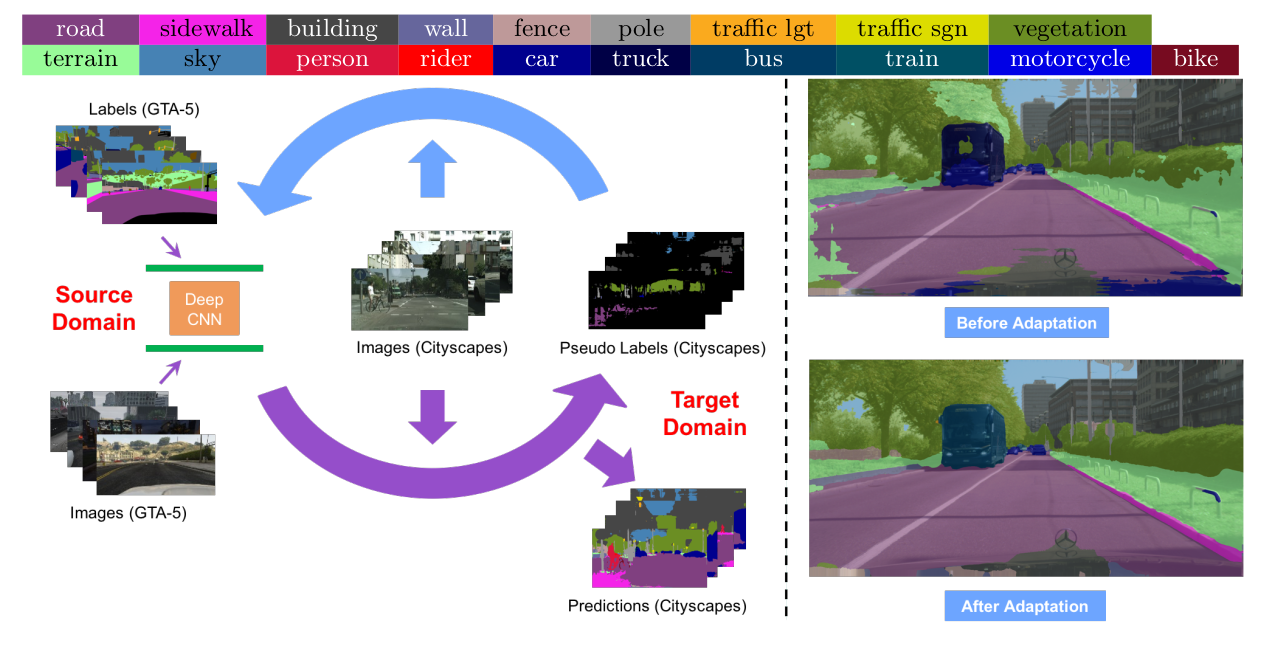
\includegraphics[width=0.8\textwidth]{Figures/From articles/semantic_segmentation.png}
    \caption{ On the left side, the self-training framework for UDA is presented. On the right side, obtained results before and after adaptation for the Cityscapes dataset.}
    \label{fig: sem_seg}
\end{figure}

The CBST approach is based on two main components: a class-balancing strategy and a self-training algorithm. The class-balancing strategy aims to address the problem of class imbalance between the source and target domains, which can negatively impact the performance of the segmentation model. The authors change the loss function using parameters that determine the proportion of selected pseudo-labels due to balance the class distribution during the self-training process. Furthermore, when the images in the source and target domains are similar, spatial prior knowledge can be effectively utilized to adapt models. For this purpose, the authors count the class frequencies in the source domain using Gaussian kernel. The experimental results show that the CBST approach outperforms several state-of-the-art unsupervised domain adaptation methods for semantic segmentation. 